%%%%%%%%%%%%%%%%%%%%%%%%%%
%%% author : Yamada. T %%%
%%% made for TH series %%%
%%%%%%%%%%%%%%%%%%%%%%%%%%

\documentclass[b5paper,10pt,fleqn] {ltjsarticle}

\usepackage[margin=10truemm]{geometry}

\usepackage{pict2e, graphicx}
\usepackage{tikz}
\usetikzlibrary{intersections,calc,arrows.meta}

\usepackage{amsmath, amssymb, amsthm}
\usepackage{ascmac}
\usepackage{comment}
\usepackage{empheq}
\usepackage[shortlabels,inline]{enumitem}
\usepackage{fancybox}
\usepackage{fancyhdr}
\usepackage{here}
\usepackage{lastpage}
\usepackage{listings, jvlisting}
\usepackage{fixdif}

\usepackage{stmaryrd}
\usepackage[listings]{tcolorbox}
%\usepackage{ascolorbox}
\usepackage{titlesec}
\usepackage{ulem}
\usepackage{url}
\usepackage{verbatim}
\usepackage{wrapfig}
\usepackage{xcolor}
\usepackage{luatexja-ruby}
\usepackage{varwidth}
\usepackage[version=3]{mhchem}
\usepackage{wrapfig}


\usepackage{physics2}
	\usephysicsmodule{ab}
	\usephysicsmodule{ab.braket}
	\usephysicsmodule{ab.legacy}
	%\usephysicsmodule{braket}
	\usephysicsmodule{diagmat}
	\usephysicsmodule{xmat}
	\usephysicsmodule{nabla.legacy}
	\usephysicsmodule{qtext.legacy}

\usepackage[ISO]{diffcoeff}
\difdef { f, s } { D }
{ op-symbol = \mathrm{D} }


\newcommand{\mctext}[1]{\mbox{\textcircled{\scriptsize{#1}}}}
\newcommand{\ctext}[1]{\textcircled{\scriptsize{#1}}}
\newcommand{\ds}{\displaystyle}
\newcommand{\comb}[2]{{}_{#1}\mathrm{C}_{#2}}
\newcommand{\hs}{\hspace}
\newcommand{\vs}{\vspace}
\newcommand{\emphvs}{\vspace{1em}\notag\\}
\newcommand{\ora}{\overrightarrow}
\newcommand{\ol}{\overline}
\newcommand{\oramr}[1]{\overrightarrow{\mathrm{#1}}}
\newcommand{\tri}{\triangle}
\newcommand{\mr}{\mathrm}
\newcommand{\mb}{\mathbb}
\newcommand{\mrvec}[1]{\overrightarrow{\mathrm{#1}}}
\newcommand{\itvec}{\overrightarrow}
\newcommand{\bs}{\boldsymbol}
\newcommand{\ra}{\rightarrow}
\newcommand{\Ra}{\Rightarrow}
\newcommand{\lra}{\longrightarrow}
\newcommand{\Lra}{\Longrightarrow}
\newcommand{\la}{\leftarrow}
\newcommand{\La}{\Leftarrow}
\newcommand{\lla}{\longleftarrow}
\newcommand{\Lla}{\Longleftarrow}
\newcommand{\lr}{\leftrightarrow}
\newcommand{\llr}{\longleftrightarrow}
\newcommand{\Llr}{\Longleftrightarrow}
\renewcommand{\deg}{{}^\circ}
\newcommand{\phbox}{\fbox{\phantom{1\hspace{2em}}}}
\newcommand{\boxnum}[1]{\fbox{\phantom{\hspace{1em}}({#1})\phantom{\hspace{1em}}}}
\newcommand{\boxkana}[1]{\fbox{\phantom{\hspace{1em}}{#1}\phantom{\hspace{1em}}}}
\newcommand{\boxkm}[2]{\fbox{\, {#1}\phantom{\hspace{0.2em}} \,  {#2}}}
\newcommand{\hzw}{\hspace{1\zw}}

\renewcommand{\baselinestretch}{1.25}
\parindent=1\zw

%TH3-1
\begin{document}
\noindent\fbox{NewTH1-3} [京都大]

次の文を読んで,空欄に適した式を記せ.必要であれば三角関数の公式$\sin 2\theta = 2 \sin \theta \cos \theta$を用いること.

\begin{wrapfigure}{r}{9cm}
  \centering
  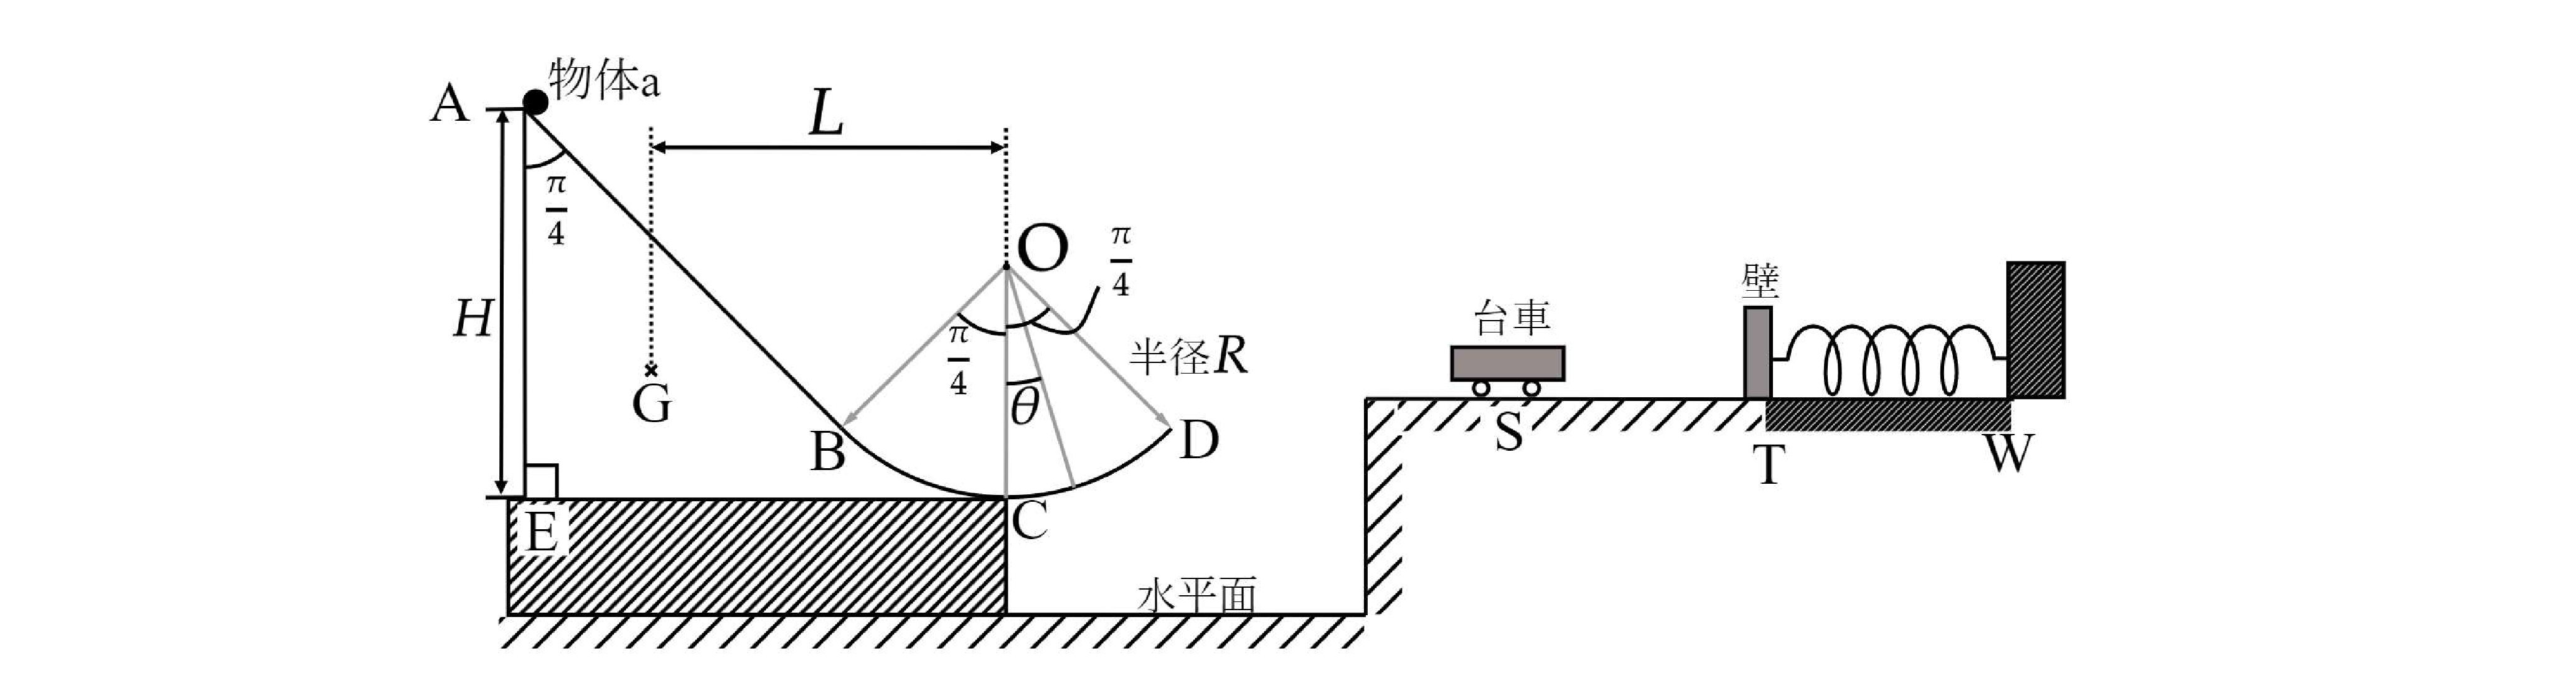
\includegraphics[width=9cm]{fig/fig_1_3.pdf}
\end{wrapfigure}
水平面上に質量が十分に大きい直方体の台(右図の斜線部)があり,その台上に,側面がABCEで表される質量$M$のすべり台を置いた.ABは直線であり,BCは半径$R$の円弧である.すべり台の先端(点C)には,図のように質量の無視できる半径$R$の円弧CDの板が取り付けられており,すべり台と円弧CDは剛体として一体となって動く.すべり台と円弧CDの厚み(図では紙面と垂直な方向の長さ)は考えないものとする.また,半径OBとOC,およびOCとODのなす角度はそれぞれ$\ds\frac{\pi}{4}$である.直方体の台と水平面の間,およびすべり台と直方体の台の間には摩擦力が働き,水平方向には動かないものとする.

 点Aは直方体の台の上面から高さ$H$の位置にある.Aから,大きさの無視できる質量$m$の物体aが斜面をすべり落ち,半径$R$の円弧BCDの区間を通って点Dから空中に放出された.$H > R$とし,斜面ABおよび円弧BCDはなめらかであるとする.また,重力加速度の大きさを$g$とし,空気抵抗は無視できるものとする.

\begin{enumerate}[I]
  \item \hzw 物体aが円弧CDを通過するとき,すべり台(ABCEの部分)が点Cを中心として回転し,浮き上がるかどうかを考えよう.

  \hzw まず,物体aが円弧CDに及ぼす力による点Cのまわりの力のモーメントを計算する.物体aが半径OCから円弧CDの方向に測って角度$\theta\ \ab(0 \leqq \theta \leqq \dfrac{\pi}{4})$の位置にあるとき,物体aの速度の大きさを$H$,$R$,$g$,$\theta$を用いて表すと\boxnum{1}となる.また,物体aが円弧に及ぼす力の大きさを$H$,$R$,$g$,$\theta$,$m$を用いて表すと\boxnum{2}となり,
  \begin{gather*}
    \theta = \text{\boxnum{3}}
  \end{gather*}
  の位置で最大となる. 点Cのまわりの力のモーメントは,右回り(時計回り)を正とすれば,$H$,$R$,$g$,$\theta$,$m$を用いて\boxnum{4}と表され,
  \begin{gather*}
    \theta = \text{\boxnum{5}}
  \end{gather*}
  の位置で最大となる.
  
  \hzw 一方,すべり台の重心の位置は図中の点Gであり,点Gと点Cの水平距離を$L$とする.すべり台の質量による点Cのまわりの力のモーメントは,左回り(反時計回り)を正とすれば$MgL$となるので,すべり台が浮き上がらない条件は,
  \begin{gather*}
    MgL \geqq \text{\boxnum{6}} \ \text{((4)の最大値)}
  \end{gather*}
  で与えられる.
  
  \item \hzw 物体aは点Dで空中に放出された後,点Dと同じ高さの水平な床面上においてある,大きさが無視できる質量$m$の台車に点Sで衝突した.点Dと点Sの距離を$H$,$R$を用いて表すと\boxnum{7}となる.

  \hzw 物体aは点Sで台車と完全非弾性衝突し,衝突後一体となり質量$2m$の物体bとして床面の上を水平方向に動いた.ただし,点Tまで床はなめらかであり,台車と床との間に摩擦力は働からないものとする.そのときの物体bの速度の大きさ$V$は,$H$,$R$,$g$を用いて,
  \begin{gather*}
    V = \text{\boxnum{8}}
  \end{gather*}
  となる.

  \hzw 物体bはばねのついた質量$m$の壁に完全非弾性衝突し,物体bと壁は一体となって,質量$3m$の物体cとして動き出した.衝突前のばねの長さは自然の長さであった.衝突直後の物体cの速度の大きさ$U$は,$V$を用いて表すと\boxnum{9}となる.

  \hzw 物体cが動き出した後,TWの区間内では質量$3m$の物体cと床面の間に摩擦力が働くものとし,そのときの静止摩擦係数$\mu_0$,動摩擦係数は$\mu$である.物体bが壁に衝突してから,物体cが最初に速度0となったときのばねの縮み量を$\varDelta l$とおく.ばね定数を$k$とすると,$\varDelta l$は$U$,$m$,$g$,$\mu$,$k$を用いて\boxnum{10}となる.また,ばねが$\varDelta l$だけ縮んだ位置から再び動き出さないための条件式は,
  \begin{gather*}
    k\varDelta l \leqq \text{\boxnum{11}}
  \end{gather*}
  となる.
\end{enumerate}

\end{document}

